\chapter{Búsqueda en espacios de estados}

\section{Diseño de un agente deliberativo: Búsqueda}

Los \textbf{agentes deliberativos} disponen de un modelo del mundo en el que habitan y de los efectos de sus acciones sobre dicho mundo.
Trabajando con ambos modelos, estos agentes pueden razonar sobre ellos para decidir qué hacer para conseguir un objetivo.

\subsection{La búsqueda en un espacio de estados}

Un \textbf{espacio de estados} es la representación del conocimiento a través de las acciones del agente.
Una \textbf{búsqueda en el espacio de estados} es una resolución del problema mediante la proyección de las distintas acciones que éste realiza.

\subsection{Ejemplo de un agente deliberativo: El mundo de bloques}

Supongamos un mundo cuadriculado con tres bloques $A$, $B$ y $C$.
Modelamos este mundo como una secuencia de listas de objetos sobre objetos, siendo el \textbf{estado inicial} \code{[[A],[B],[C]]}.
Si tuviéramos el bloque $B$ sobre el bloque $A$ y el bloque $C$ en el suelo sin estar en contacto con los otros, el estado sería \code{[[B,A],[C]]}.

El \textbf{objetivo} del agente es apilar los bloques de forma que $A$ quede sobre $B$, que debe quedar sobre $C$, con este último en el suelo.
Buscamos el \textbf{estado destino} \code{[[A,B,C]]}.
Para conseguir esto, el agente cuenta con la función \code{mover(x,y)} para colocar un bloque \code{x} sobre otro bloque \code{y} para $x={A,B,C}$ e $y={A,B,C,Suelo}$.
Asumimos que se descartan llamadas imposible de esta función, como aquellas en la sque se cumple que $x=y$ o mover bloques que se encuentren debajo de otros.
En este caso, el \textbf{coste} de todas las acciones es el mismo.

Para buscar las acciones que nos lleven al objetivo final podemos usar un \textbf{grafo de estados}, que es un grafo dirigido en el que cada nodo represente un estado del sistema y cada lado la acción que debe realizar el agente para pasar de un estado a otro.

Llamamos \textbf{plan} a la secuencia de acciones dentro del grafo de estados que lleva al agente del estado inicial al estado destino, siendo la búsqueda de dicha secuencia su \textbf{planificación}.

\begin{center}
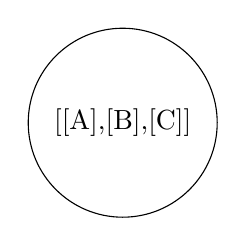
\begin{tikzpicture}[scale=0.2]
\tikzstyle{every node}+=[inner sep=0pt]
\draw [black] (6.2,-6.2) circle (6);
\draw (6.2,-6.2) node {\code{[[A],[B],[C]]}};
\end{tikzpicture}
\end{center}

\section{Sistemas de búsqueda y estrategias}

\section{Búsqueda sin información}

\section{Búsqueda con información}

\section{Problemas descomponibles y búsqueda}
